\subsection{Deterministic Parallelism}\label{sec:eval-parallelism}
%=============================================================================

%% \RN{Remember: Figure % \ref{fig:eval-summary} and
%%   \ref{fig:laws} needs to be updated.}

Finally, we evaluate our Liquid Haskell deterministic
parallelism prototypes.  Aside the lines of proof code added, it is also
necessary to evaluate the impact on runtime performance.
%
Were we using a proof tool external to Haskell, this would not be necessary.
But our proofs are Haskell programs---they are necessarily visible to the
compiler.  In particular this means a proliferation of unit values and functions
returning unit values.  Also, verified instances are witnessed at runtime by
``dictionary'' data structures passed between functions.  Layering them on top
of existing clases like @Ord@ could potentially add indirection or change the
code generated, depending on the details of the optimizer.
%
% Whole program compiler would be especially well suited
%
%% We do some evaluation to claim that verification has little to no effect on
%% runtime performance.
In our experiments we find little or no effect on runtime performance.
Benchmarks were run on a single-socket Intel{\textregistered}
Xeon{\textregistered} CPU E5-2699 v3 with 18 physical cores and 64GiB RAM.

\subsubsection{LVish: Concurrent Sets}
\label{sec:set}

% \RGS{What are PureSet and SLSet here? Needs context.}
We benchmark concurrent sets storing 64-bit integers.
%% Here we aim to maximize overhead by repeatedly calling the function
%% with @VerifiedOrd@
We measure the total time for a fixed number of parallel @insert@ operations
against parallel @verifiedInsert@ operations, varying the number of concurrent
threads, and plotting the parallel speedup. The results are shown in
Figure~\ref{fig:set}. There is a slight observable difference between the two
lines because the extra methods still exist at runtime.
%
We repeat the experiment for two set implementations: a concurrent skiplist
(SLSet) and a purely functional set inside an atomic reference (PureSet).

% \NV{What is HasPut? ISet, Par}
% \NV{Add reference to Fig 10 and say with words what you conclude from this fig. ie
% how proof obligations affect speedups}
% \NV{Other than speed ups we should comment on proof burden that is added when we write verifiedInsert
% instead of insert.
% Maybe how many lines of code verified Insert and insert are?}

\begin{figure}
%  \vspace{-20mm}
  \begin{center}
    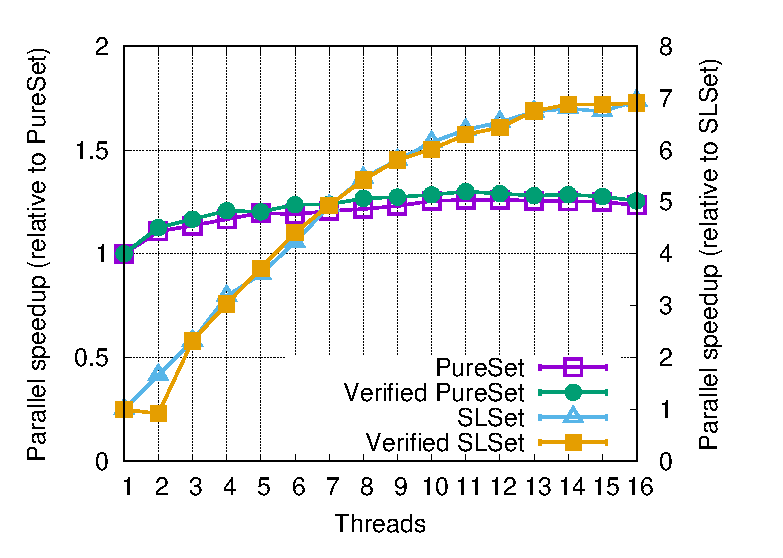
\includegraphics[width=3.2in]{text/refinementreflection/set.eps}
  \end{center}
  \caption{Parallel speedup for doing 1 million parallel inserts over 10
    iterations, verified and unverified, relative to the unverified version,
    for PureSet and SLSet}
  \label{fig:set}
\end{figure}

\subsubsection{\texttt{monad-par}: $n$-body simulation}
\label{sec:nbody}

We noted in \S~\ref{sec:detpar} that Liquid Haskell proofs can scale up to
larger algebraic datatypes. We demonstrate an example of this by verifying an
$n$-body simulation program that leverages @monad-par@, a Haskell library which
provides deterministic parallelism for pure code \cite{monad-par}.

An $n$-body simulation is used to model the behavior of particles in some system
in which forces are acting on the particles. The code which we verify is adapted
from an implementation of the all-pairs variant (a traditional, brute-force
approach) to $n$-body simulation from \cite{parallel-n-body}. The datatype which
we are verifying represents a particle:

\begin{code}
data Body = Body Double Double Double Double
                 Double Double Double
\end{code}

That is, a seven-tuple of @Double@s. When updating a @Body@'s velocity from the
acceleration due to other particles exerting force on the @Body@, there is a
special case when both particles are the same:

\begin{code}
  accel :: Body -> Body -> Accel
  accel b_i b_j
    | b_i <= b_j && b_j <= b_i = Accel 0 0 0
    | otherwise = ...
\end{code}

To ensure that @accel@ is deterministic, we wish to verify that the @<=@ function
here is really a total order (i.e., a @VerifiedOrd@). As noted earlier, we already
have a @VerifiedOrd (a, b)@ instance, and writing a @VerifiedOrd Double@ instance
is simple, so writing a @VerifiedOrd Body@ instance is as simple as writing:

\begin{code}
type BodyRep = (Double, (Double, (Double,
  (Double, (Double, (Double, Double))))))
instance Iso Body BodyRep
\end{code}

Figure~\ref{fig:nbody} demonstrates the results of running the $n$-body simulation
with two differences: one uses the standard, unverified @Ord@ typeclass, and one
uses @VerifiedOrd@. It is worth noting that the runtime performance of the two
versions of the program are almost identical, despite the difference in behavior
between @accel@, which is run in a loop.
This demonstrates that it is possible
to verify even performance-critical code without incurring substantial performance
penalties.

\begin{figure}
  \begin{center}
    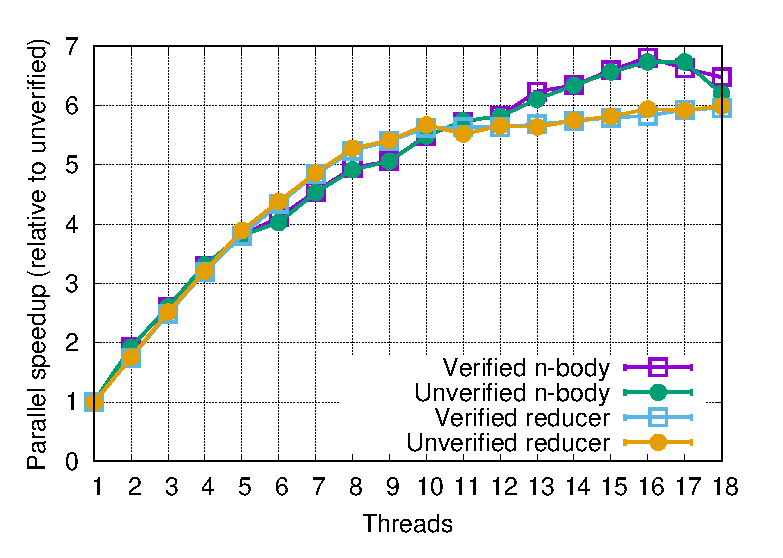
\includegraphics[width=3.2in]{text/refinementreflection/nbody.eps}
  \end{center}
  \caption{Parallel speedup for doing a parallel $n$-body simulation with
    1,024 bodies and 20 iterations, verified and unverified, relative to the
    unverified version}
  \label{fig:nbody}
\end{figure}

\subsubsection{DPJ: Parallel Reducers}
\label{sec:reducer}

The Deterministic Parallel Java (DPJ) project provides a deterministic-by-default
semantics for the Java programming language \cite{DPJ}. In DPJ, one can declare a
method as @commutative@, e.g.,
%
% \begin{lstlisting}[language=java]
\begin{code}
private region AccumRgn;
private static int sum in AccumRgn;
private static commutative synchronized
  void updateSum(int n) writes AccumRgn
   { sum += n; }
\end{code}
%\end{lstlisting}
%
This asserts that racing calls to @updateSum@ have the same observable effect.
%% to express the property that the operation in that when the method is executed
%% several times, any ordering of the methods is permitted.
%
While a parallel fold of a known input space needs only associativity, a {\em
  reducer variable}, such as @sum@ above, must cope with any number of updates
coming from any number of threads.
%% Commutativity of operations is essential to many classes of parallel
%% programs. For example, doing a parallel reduction of an array of integers
%% requires that the reduction operation be commutative, lest the result of the
%% reduction become nondeterministic.
%% \RN{That doesn't distinguish it from a fold though...}

However, the @commutative@ keyword simply states an invariant. That is, DPJ does not perform
any kind of check to ensure that a method marked @commutative@ does, in fact,
actually commute. With Liquid Haskell, however, we can build fully-verified
parallel reducer variables, by proving commutativity.

To express the above parallel reducer code in Liquid Haskell, we need a type for
{\em reduction variables} which use a binary operation (from @Monoid@) to
combine values received.  Because we need commutativity as well, we must prove
@VerifiedAbelianMonoid@:

%% will need a data
%% structure for the result, as well as an operation over it. We will use:
%% \RN{appendSum seems very unintuitive for the average reader.  Changing.}
\begin{code}
 newtype RVar s a
 newRVar :: VerifiedAbelianMonoid a
         => Par s (RVar s a)
 updateRVar :: a -> RVar s a -> Par s ()

 class VerifiedMonoid a =>
       VerifiedAbelianMonoid a where
  commutes :: x:a -> y:a -> {x<>y = y<>x}
\end{code}

%% \begin{code}
%% newtype Sum = Sum { getSum :: Int }
%% reflect plus :: Sum -> Sum -> Sum
%% plus :: Sum -> Sum -> Sum
%% plus x y = Sum (getSum x + getSum y)
%% \end{code}

%% We want addition of @Sum@s
%% % (which we dub @appendSum@)
%% to commute.  We can extend the @VerifiedMonoid@ class with the property we
%% desire:

%% \begin{code}
%% class VerifiedMonoid a =>
%%       VerifiedAbelianMonoid a where
%%   commutes :: x:a -> y:a -> { x <> y = y <> x }
%% \end{code}

In the DPJ example above, we compute a sum, which uses the natural
@VerifiedAbelianMonoid@ instance for integers.  A reduction variable typically
has either one replica, or a replica per thread, but this is now provably
transparent to the user of the API.  Thus we no longer need to trust the programmer,
as in the DPJ example above.

%% Since @Sum@ is a simple wrapper around an integer addition, it is quite simple to
%% prove the commutativity of @plus@, so we elide the proof here. (The proofs of
%% associativity and identity laws are similarly straightforward). Now
%% we need a computation that requires the use of these properties, which we will
%% call @updateRef@:

%% \begin{code}
%% updateRef :: VerifiedAbelianMonoid a
%%           => IORef a -> a -> IO ()
%% updateRef ref partialS
%%   = atomicModifyIORef' ref $ \sum ->
%%       (sum <> partialS, ())
%% \end{code}

% \RGS{Should updateRef be simplified for presentation purposes?}
% \RN{Yes, I think what we're ultimately going for is NOT IO.}

%% Here, the @ref@ is a mutable reference to some value of type @a@, and we use
%% @atomicModifyIORef'@ to retrieve the contents of @ref@ and update the value of
%% @ref@ to be the result of the verified semigroup operation, given arguments of
%% the original value of @ref@ and @partialS@.

%% This is analogous to the
%% @sum += partialS@ line from the DPJ code, but with a static guarantee that @+=@
%% must be commutative.
%% Now we are free to call @updateRef@ in parallel from many threads, all of which
%% reduce a segment of an array sequentially and then update a shared @IORef@ value
%% using @updateRef@.

In Figure \ref{fig:nbody} we evaluate a simple version of this program.  We
update a single, global reduction variable using a varying number of threads.
Each thread sums segments of an array, sequentially, and updates the reduction
with these partial sums.
%
%% The results of running this program with varying numbers of
%% threads are shown in Figure \ref{fig:reducer}.
%
Once again, we ran verified against unverified and observed no appreciable
difference in performance.

%%% Local Variables:
%%% mode: latex
%%% TeX-master: t
%%% End:
